\documentclass[tikz]{standalone}
\usepackage{tikz}
\usetikzlibrary{positioning, graphs}
\usetikzlibrary{graphs.standard}
\begin{document}
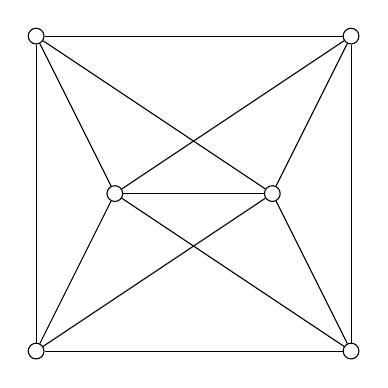
\begin{tikzpicture}
		[vertex/.style={draw,circle,inner sep = 0mm, minimum size = 2mm},
		 edgelabel/.style = {fill = white, inner sep = 0mm, font=\tiny}]
		\node[vertex] at (-2,2)	 (a) {};
		\node[vertex] at (2,2)	 (b) {};
		\node[vertex] at (-1,0)	 (c) {};
		\node[vertex] at (1,0)	 (d) {};
		\node[vertex] at (-2,-2) (e) {};
		\node[vertex] at (2,-2)	 (f) {};
		
		\draw (a) -- (b);
		\draw (a) -- (c);
		\draw (a) -- (d);
		\draw (a) -- (e);
		\draw (b) -- (c);
		\draw (b) -- (d);
		\draw (b) -- (f);
		\draw (c) -- (d);
		\draw (c) -- (e);
		\draw (c) -- (f);
		\draw (d) -- (e);
		\draw (d) -- (f);
		\draw (e) -- (f);
\end{tikzpicture}
\end{document}